\documentclass[11pt]{article}
\usepackage[english]{babel}
\usepackage{inputenc}
\usepackage{multicol}
\usepackage{flushend}
\usepackage{fullpage}
\usepackage{graphicx}
\usepackage{epsfig}
\usepackage{caption}
\captionsetup[table]{labelsep=period}
\usepackage{multirow}
\usepackage{mathtools}
\usepackage{xcolor}
\DeclarePairedDelimiter{\ceil}{\lceil}{\rceil}

\topmargin=-0.2in
\textheight=9.5in

\pagestyle{empty}

\begin{document}

\centerline{CSCE 614 (Fall 2020) \hfill Uwacu and Elsheimy}
\medskip
\centerline{\bf Computer Architecture}
\medskip

\centerline{\bf  Project proposal: }

\bigskip

\centerline{\bf Exploring Predictive Replacemebt Policies for Instruction Cache and Branch Target Buffer}

\bigskip

\centerline{\bf Diane Uwacu and Fatmaelzahraa Elsheimy}

\bigskip

\begin{abstract}
	For our final project, we will implement a global history replacement policy for instruction cache and branch target buffer.
	The method was shown to lower instruction cache MPKI by an average of 18\% over the least recently-used policy, and it showed
	similar improvements over several other policies.
	We plan to implement and validate the results in the original work by comparing against at least one of the stated methods.
\end{abstract}

\section{Introduction} 
\label{sec:introduction}

The instruction cache (I-cache) stores blocks of recently used instructions, and the branch target buffer (BTB) caches targets of previously taken branches. 
This means that the I-cache improves throughput and latency while the BTB latency due to branch target re-computation, making them both essential.
The work in \cite{samira-ISCA18} explores efficient replacement policies at the I-cache and BTB levels. Authors propose a history-based algorithm that predicts
dead blocks that should be evicted with no penalty since they are guaranteed that they won't be reused before eviction.

Authors surveyed recent work on cache replacement and noticed that a common obervation in this research area is that sequences of recently accessed instructions
correlate with the likelihood of block reuse. With this knowledge, they developed the Global History Reuse Prediction (GHRP) to predict reuse behaviors in I-cache and BTB.

Authors evaluated seven recent replacement policies and discussed their effect on the I-cache and BTB hit rates and did a comparison based average MPKI values.
Authors validated their work and run comparative analysis using benchmarks from the fifth Championship Branch Prediction Competition (CBP-5) \cite{cbp-5}.
With their experimental evaluation, they were able to explain why sampling-based replacement policies failed to improve things on the I-cache and BTB level.

For our final project, we would like to implement the GHRP replacement policy and run it through the CBP-5 benchmarks. Time allowing, we would like to compare our 
results to one of the methods that the original paper compared against.

\section{Background}
\label{sec:background}

According to authors, not much work has been done to evaluate replacement policies on the I-cache and BTB level. Except for the work in \cite{smith-1985} that was done in the 80s
with simpler policies like FIFO, and the work by Perleberg et al \cite{perleberg-1993} from the 90s, this is the first recent work to look at this problem from this angle.

Authors discuss how different prediction replacement policies affect and are affected by the I-cache and BTB. In particulat, they showed how a sampling-based
prediction policy that works well for PC-based dead block prediction, does not work as well in this area, due to the fact that a given PC only accesses one set at a time.
In addition to the sampling-based method, authors compare their work againt the least recently-used (LRU) policy, the random policy, and the static re-reference predictor (SRRIP).

\section{Motivation}
\label{sec:motivation}

Most other publications has only considered enhancing prefetching methods or software-based approaches. We are focusing our 
effort on improving replacement policies in I-cache and BTB based on dead-block prediction. When looking at recent work studying 
the effect of replacement policy, not many were found or mostly gave poor results, . Most of them focused on different approaches 
such as recent static prediction and using a hashed value for indexing branch predictors table. Other works that studied dead-block 
prediction mainly focused on using it in power reduction or bypassing. Hence, our efforts will be focus on studying the use of dead block prediction
in the I-cache and BTB. Different algorithms will be tested to be able to adapt the dead block information to BTB and I-cache replacement using open-source simulator.  

\section{Proposed technique}
\label{sec:proposed}
1.	Find a proper open-source simulator that could be used to study BTB and I-cache.
2.	Modify the simulator by adding appropriate code to collect the necessary data for studying
3.	Implement a replacement algorithm that uses the past history to predict dead-blocks in cache and BTB
4.	Implement a 64kB I-cache with a 64B block size.
5.	Implement three prediction tables with 4096 entires and a two-bit counter per entry- it will be used for predicting the dead blocks and dead entries in BTB.
6.	Measure performance of our modified simulator using LRU as baseline and studying MPKI values
7.	Compare our modified simulator with another state of art approach by studying the MPKI values


\section{Estimated timeline}
\begin{figure}[h]
	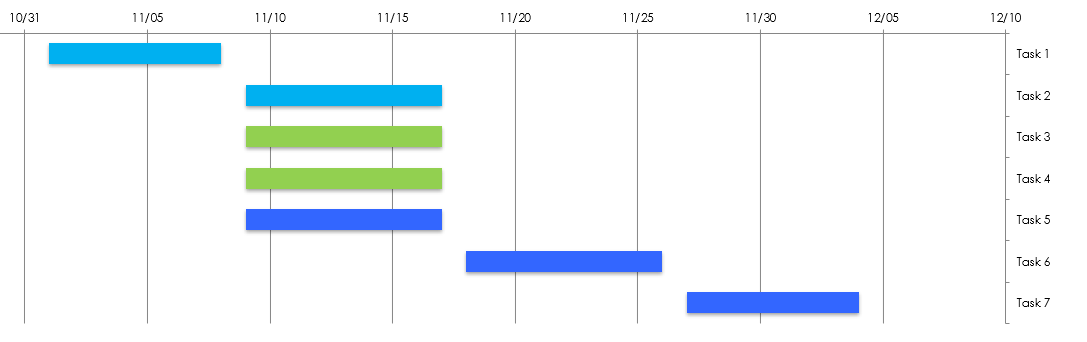
\includegraphics[width=1\textwidth]{Timeline.PNG}
\end{figure}
\label{sec:timeline}




{%\scriptsize
	\bibliographystyle{abbrv}
	\bibliography{references}
	}

\end{document}



